\section{Euler: The Bridge from Circles to Exponentials (1748)}


\section{Euler: The Exponential Bridges Everything (1740s)}

If Newton found calculus in series, and Leibniz turned it into a grammar, \textbf{Leonhard Euler} revealed its secret melody: the exponential function.

For Euler, the constant \( e \) wasn’t just a number—it was the gateway to something deeper. He saw that \( e \) was simply the value of the exponential function at \( x = 1 \):

\[
e^x = \sum_{n=0}^{\infty} \frac{x^n}{n!}
\]

The real hero wasn’t \( e \) itself, but the entire exponential function \( e^x \). Why? Because it let you solve differential equations—the equations that describe change, growth, decay, oscillation, and diffusion. The exponential function wasn’t just a formula—it was a universal key.

\vspace{1em}

\subsection{A Function That Solves Itself}

Euler noticed something remarkable: the exponential function is its own derivative:

\[
\frac{d}{dx} e^x = e^x
\]

This seemingly simple fact made it the natural solution to countless differential equations. Every time a process changed proportionally to its current value—radioactive decay, compound interest, population growth—the exponential function was quietly at work.

\vspace{1em}

\subsection{The Path to Imaginary Numbers}

To appreciate Euler’s formula, we need to take a step back. Today, \( i \), the square root of \(-1\), feels almost mundane—a symbol we manipulate without hesitation. But in Euler’s time, it was a strange and unsettling idea.

The seeds of imaginary numbers were planted by Italian algebraists in the 16th century, like \textbf{Cardano}, who encountered square roots of negative numbers when solving cubic equations. At first, these quantities were dismissed as “sophistic” or “useless”—ghosts of algebraic manipulation that couldn’t correspond to anything real.

By the 17th century, mathematicians like \textbf{Bombelli} and \textbf{Descartes} (who coined the term “imaginary”) began to cautiously explore their properties. Yet they still seemed algebraically valid but geometrically meaningless.

Then came the great conceptual leap: realizing that imaginary numbers weren’t just nonsensical algebra—they could be understood as \emph{directions perpendicular to the real line}. In the early 18th century, mathematicians like \textbf{Argand}, \textbf{Wessel}, and later \textbf{Gauss} gave geometric interpretations of complex numbers as points in a plane, with the real part on the horizontal axis and the imaginary part on the vertical.

Euler stood at the cusp of this transformation. He realized that multiplying by \( i \) wasn’t just algebra—it was a rotation by 90 degrees in this complex plane. And if \( i \) rotated once, then \( i^2 = -1 \) rotated again, flipping to the opposite real direction.

\vspace{1em}

\subsection{Extending the Exponential}

Once Euler had the geometric intuition of complex numbers as points in a plane, he asked a bold question:

\begin{quote}
\textit{What happens if we extend the exponential function to imaginary inputs?}
\end{quote}

After all, the exponential \( e^x \) could already be defined by its power series:

\[
e^x = 1 + x + \frac{x^2}{2!} + \frac{x^3}{3!} + \cdots
\]

So why not simply let \( x = i\theta \) and substitute?

\[
e^{i\theta} = 1 + i\theta + \frac{(i\theta)^2}{2!} + \frac{(i\theta)^3}{3!} + \cdots
\]

When he expanded this series and grouped the real and imaginary terms, something miraculous appeared:

\[
e^{i\theta} = \left(1 - \frac{\theta^2}{2!} + \frac{\theta^4}{4!} - \cdots\right) + i\left(\theta - \frac{\theta^3}{3!} + \frac{\theta^5}{5!} - \cdots\right)
\]

But these series were already known—they were the Taylor expansions for cosine and sine! Thus:

\[
e^{i\theta} = \cos \theta + i \sin \theta
\]

Euler’s formula wasn’t a lucky coincidence—it was the inevitable consequence of extending the exponential into the complex world.

\vspace{1em}

\begin{center}
\textit{Where the square root of \(-1\) once seemed a mathematical ghost, Euler revealed it as a rotation in an invisible plane.}
\end{center}



\subsection{The Bridge to Trigonometry}

But Euler’s most astonishing discovery wasn’t just about solving equations—it was about connecting worlds. He found that the exponential function could describe rotation, by letting \( x \) be imaginary:

\[
e^{ix} = \cos x + i \sin x
\]

This equation—now known as \textbf{Euler’s formula}—wove together algebra, geometry, trigonometry, and analysis in a single, elegant thread. Through it, waves, rotations, and oscillations became different faces of the same exponential function.


\vspace{1em}

\begin{HistoricalSidebar}{From Heat to Randomness}

The exponential function didn’t stop at circles and waves. It also appeared in diffusion, through solutions to the \textbf{heat equation}. The heat kernel—describing how heat spreads from a point—has the shape of a normal distribution whose variance grows over time. And as heat spreads, probability follows: the same exponential underpins the \textbf{central limit theorem}, explaining why randomness converges to a bell curve.

It also unlocked new ways of thinking about Fourier series: whether as sums of sines and cosines, or as sums of complex exponentials. Music, signal processing, quantum mechanics—everything vibrating could now be analyzed through Euler’s lens.

Even outside deep mathematics, \( e \) sneaks into life’s puzzles:

\begin{itemize}
    \item At a chaotic coat check, if everyone randomly grabs a coat, the chance that no one gets their own is about \( \frac{1}{e} \).
    \item In love, if you expect to meet \( N \) potential partners, the optimal stopping rule is to reject the first \( \frac{N}{e} \) and choose the next one who surpasses all before.
\end{itemize}

\vspace{1em}

\begin{center}
\textit{If Newton saw calculus in series, and Leibniz in symbols, Euler heard it in the exponential’s song—a harmony uniting change, rotation, heat, and chance.}
\end{center}


If Barrow saw curves as geometric entities—measured by tangents and areas—then \textbf{Leonhard Euler} saw them as expressions waiting to be simplified. Where Barrow drew triangles, Euler wrote formulas. Where Barrow relied on proportions, Euler invoked a new kind of mathematical poetry:  
\[
e^{ix} = \cos(x) + i \sin(x)
\]

With this single equation, Euler didn’t just connect exponentials and trigonometric functions—he redefined how we think about motion, oscillation, and periodicity.

\end{HistoricalSidebar}

\subsection{From Circles to Signals}

For centuries, \textbf{trigonometry} was inseparable from geometry. Sines and cosines were lengths of lines inside a circle—tools for navigators, architects, and astronomers. But Euler asked a different question:

\begin{quote}
\textit{What if circular motion could be described not by shapes, but by growth and rotation in the complex plane?}
\end{quote}

By extending the exponential function into the realm of imaginary numbers, Euler discovered that rotation itself could be encoded algebraically. The endless sweep of a circle became a natural consequence of exponential behavior—an elegant spiral through the fabric of numbers.

\subsection{Analysis Over Diagrams}

Where Barrow’s world was drawn with careful hands, Euler’s was written with flowing symbols. He replaced geometric constructions with analytic expressions:

\[
\cos(x) = \frac{e^{ix} + e^{-ix}}{2}
\quad \text{and} \quad
\sin(x) = \frac{e^{ix} - e^{-ix}}{2i}
\]

These identities didn’t just simplify calculations—they unlocked entirely new ways of thinking:

\begin{itemize}
    \item Oscillations could now be treated as combinations of exponential functions.
    \item Problems in mechanics, astronomy, and later electrical engineering were transformed by this shift from angles to exponents.
    \item The door to \textbf{Fourier analysis}, signal processing, and quantum mechanics stood open—whether Euler knew it or not.
\end{itemize}

\begin{figure}[H]
    \centering
    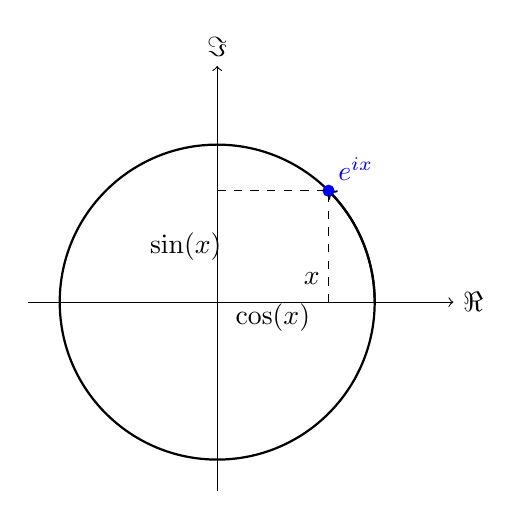
\begin{tikzpicture}[scale=2]
      % Draw unit circle
      \draw[thick] (0,0) circle (1);
      \draw[->] (-1.2,0) -- (1.5,0) node[right] {$\Re$};
      \draw[->] (0,-1.2) -- (0,1.5) node[above] {$\Im$};
      
      % Angle arc
      \draw[thick, ->] (1,0) arc (0:45:1);
      \node at (0.6,0.15) {$x$};
      
      % Point on circle
      \filldraw[blue] ({cos(45)},{sin(45)}) circle (1pt) node[above right] {$e^{ix}$};
      
      % Cosine projection
      \draw[dashed] ({cos(45)},0) -- ({cos(45)},{sin(45)});
      \node at ({cos(45)/2}, -0.1) {$\cos(x)$};
      
      % Sine projection
      \draw[dashed] (0,{sin(45)}) -- ({cos(45)},{sin(45)});
      \node at (-0.2,{sin(45)/2}) {$\sin(x)$};
    \end{tikzpicture}
    \caption{Euler’s Formula: Rotating around the unit circle becomes an exponential journey in the complex plane.}
\end{figure}

\subsection{The End of Geometric Dependence}

Euler’s work marked a turning point:

\begin{center}
\textit{Where Barrow needed diagrams, Euler needed only \( e^{ix} \).}
\end{center}

Trigonometry was no longer bound to the compass and straightedge. It had been absorbed into the algebra of exponentials—compressed into a form that could travel far beyond the page, into differential equations, wave mechanics, and the heart of modern analysis.

\vspace{1em}

Euler didn’t just compute faster—he changed what it meant to \textbf{understand} periodic motion.  
A circle, once a purely geometric object, became a manifestation of exponential behavior—an idea that still powers mathematics today.
